\chapter{Dataset Reduction}

\section{Descrizione del problema}
Lo scopo di questo elaborato è quello di analizzare un set di dati e ridurlo, in modo che sia comunque rappresentativo della popolazione da cui è stato estratto il campione.\\
Il dataset in questione contiene informazioni riguardanti parametri e valori di prestazioni di un file system di Unix, raccolte in 3000 istanze, descritte da 24 feature.\\\\
L'obiettivo, quindi, sarà quello di selezionare un numero esiguo di righe, pur mantenendo la maggior percentuale di varianza e quindi di informazione possibile.\\
Per fare questo, dopo aver manipolato preliminarmente i dati, si sono utilizzate due tecniche: la \textbf{PCA} e il \textbf{Clustering}. Come software invece sono stati utilizzati JMP e Matlab.\\\\

\section{Trattamento preliminare dei dati}
Prima di utilizzare le tecniche sopracitate, è stata calcolata la varianza di ogni colonna con JMP e il risultato è stato il seguente:\\\\\\\\\\

\begin{figure}[!h]
	\centering
	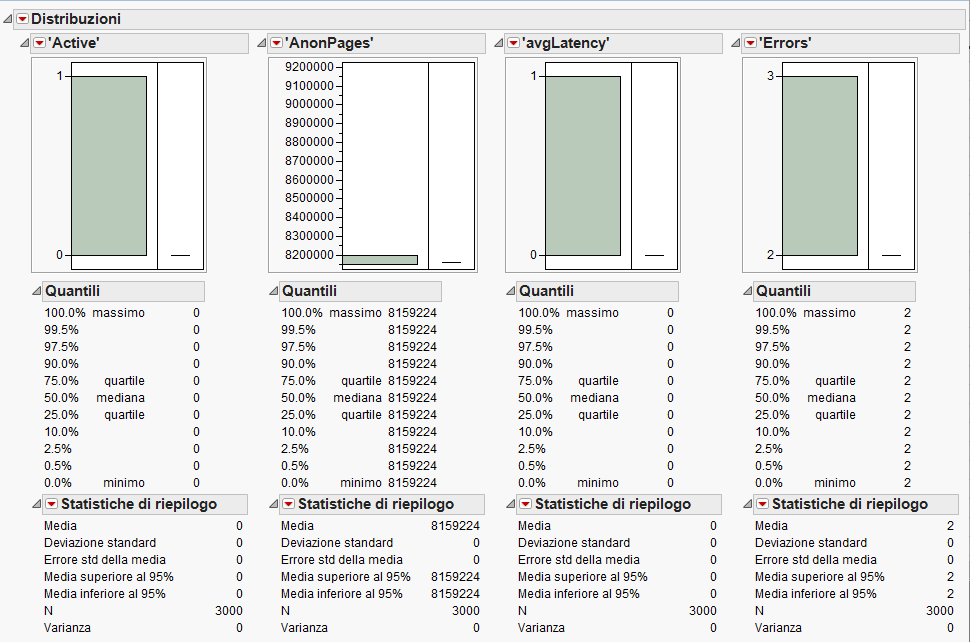
\includegraphics[width=15cm, height=10cm]{./immagine/colonne_costanti.png}
	\caption{Distribuzione colonne costanti}
	\label{fig:colonne_costanti}
\end{figure}

Come si nota sia dagli istogrammi e dal valore in basso, la varianza di queste colonne è nulla, quindi vengono eliminate in quanto non apportano contenuto informativo all'analisi dei dati.\\

\section{PCA}
Si è utilizzata la Principal Component Analysis per compiere una trasformazione lineare delle variabili originarie (gli attributi del dataset), proiettandole in un nuovo sistema cartesiano, in modo che le nuove variabili ottenute, dette \textbf{componenti principali} spieghino la maggior parte della varianza di quelle originarie.\\\\\\\\

\begin{figure}[!h]
	\centering
	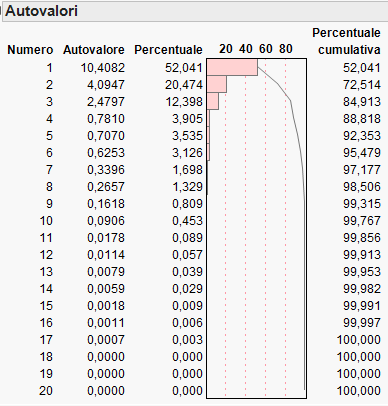
\includegraphics[width=12cm, height=10cm]{./immagine/autovalori.png}
	\caption{Componenti principali e varianza conservata}
	\label{fig:autovalori}
\end{figure}
Come si nota dalla figura esse sono ordinate in base a quanta varianza spiegano, quindi prendendo 6 componenti principali riesco a spiegare circa il 95\% della varianza.\\

\section{Clustering}
Una volta ridotto il numero di feature a 6 attraverso la PCA, si è ridotto il numero di istanze attraverso la tecnica del clustering. Quello che si fa è, una volta definita una metrica di distanza, di unire in gruppi i dati che hanno distanza minima, ovvero quelli che sono più simili.\\
Come metodo di clustering è stato scelto quello di \textbf{Ward}, che è una tecnica gerarchica agglomerativa che consiste nel formare cluster unendo ad ogni iterazione una coppia di cluster con l'obiettivo di minimizzare la varianza intra-cluster e massimizzare quella inter-cluster.\\
Il processo di clustering porta alla realizzazione della seguente struttura gerarchica detta \textbf{dendrogramma}:

\begin{figure}[!h]
	\centering
	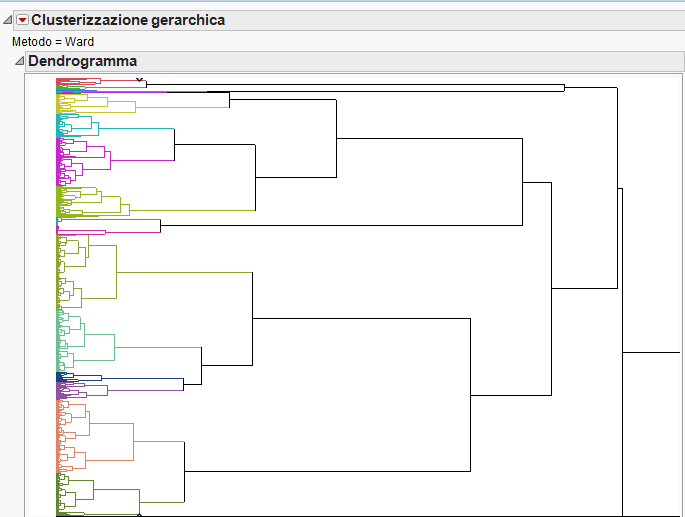
\includegraphics[width=15cm, height=12cm]{./immagine/dendrogramma.png}
	\caption{Dendrogramma}
	\label{fig:dendrogramma}
\end{figure}

Come si nota alla radice sono raggruppati tutti i dati in un unico cluster mentre, scendendo verso il basso i dati vengono divisi in più cluster fino a giungere alle foglie, che non sono altro che cluster formate da un solo elemento.\\ 
Più salgo verso la radice e più perdo varianza, più scendo verso le foglie e più la conservo, quindi bisogna trovare un trade-off tra la varianza persa e la riduzione del dataset.\\
La seguente immagine mostra la varianza persa a seconda del numero di cluster considerati:\\\\\\\\\\\\

\begin{figure}[!h]
	\centering
	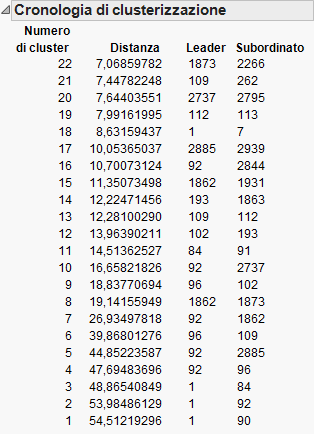
\includegraphics[width=8cm, height=10cm]{./immagine/cluster.png}
	\caption{Cluster con relativa varianza persa}
	\label{fig:cluster}
\end{figure}

In realtà si usa la devianza come metrica di distanza anzichè la varianza, in quanto vale la seguente relazione:
\begin{center}
	$devianza_{totale}=devianza_{intracluster}+devianza_{intercluster}$
\end{center} 
Quindi nella tabella precedente, ogni distanza indica la devianza persa considerando quel dato numero di cluster e calcolando il rapporto $\frac{devianza_{intracluster}}{devianza_{totale}}$, sono in grado di conoscere la percentuale di devianza e quindi di varianza (a meno di una costante) persa a seguito dell'operazione di clustering.\\\\
Si è scelto 19 come numero di cluster, poiché, superata tale soglia, si va a perdere troppa devianza cosi come si nota dal seguente grafico, dove sull'asse delle ascisse è stato messo il numero di cluster e sull'asse delle ordinate la distanza.\\\\\\\\

\begin{figure}[!h]
	\centering
	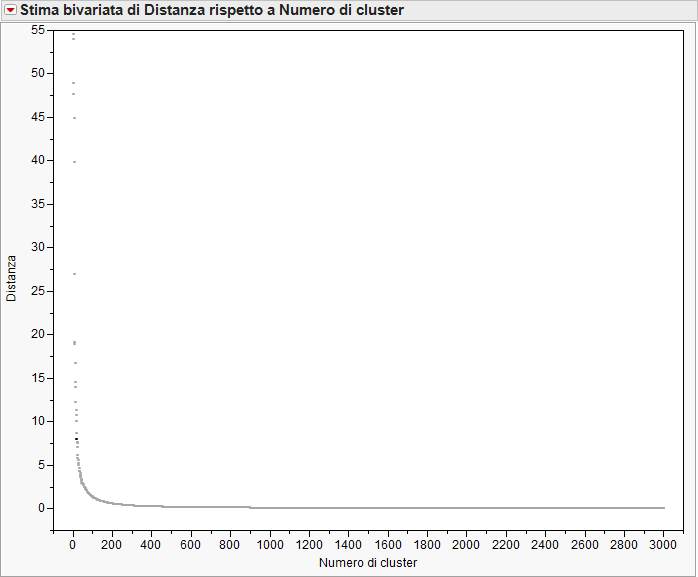
\includegraphics[width=10cm, height=10cm]{./immagine/grafico.png}
	\caption{Grafico devianza persa al variare del numero di cluster}
	\label{fig:grafico}
\end{figure} 

Scegliendo 19 cluster, quindi, perdiamo circa il 18,5\% della varianza del dataset originale e ne conservo l'81,5\%.\\\\\\\\\\\\\\\\\\\\\\

\section{Conclusioni}
In conclusione riportiamo il numero di dati che ogni cluster contiene con la relativa percentuale di copertura del dataset originario:\\

\begin{figure}[!h]
	\centering
	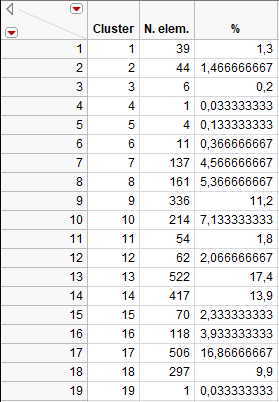
\includegraphics[width=8cm, height=10cm]{./immagine/cluster_size.png}
	\caption{Numero di elementi per ogni cluster}
	\label{fig:cluster_size}
\end{figure}

Come si nota dalla tabella ci sono alcuni cluster che contengono pochi elementi, ad esempio il cluster 19 ne contiene solo 1 e questo corrisponde all'istanza che presenta l'unico valore diverso da zero dell'attributo \textit{Slab}. Probabilmente in questi casi si tratta di \textbf{outlier}, cioè valori anomali, ma nonostante questo non sono stati eliminati in quanto potrebbero rappresentare un comportamento specifico del sistema preso in esame e quindi non avendo informazioni sulla loro significatività si è ritenuto opportuno mantenerli nel dataset.\\\\\\\\\\\\
Infine riportiamo i dati scelti in maniera casuale da ogni cluster (un elemento per ognuno), che sono rappresentativi del dataset originario.\\\\

\begin{figure}[!h]
	\centering
	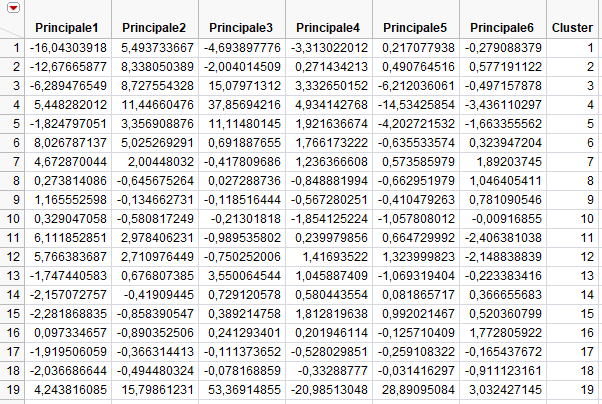
\includegraphics[width=15cm, height=13cm]{./immagine/final_data.png}
	\caption{Dati finali}
	\label{fig:final_data}
\end{figure}

